\chapter{Las estructuras de Lewis y la geometría de las moléculas}\label{ch:g10:lewis-and-shape}

Una \omterm{def:g7:atoms-and-molecules:molecule}{molécula} de dióxido de carbono es lineal; una \omterm{def:g7:atoms-and-molecules:molecule}{molécula} de agua es
angular. Esa sola diferencia de forma es una de las razones por las que
el agua, con \omterm{def:g7:atoms-and-molecules:molecule}{moléculas} más ligeras que las del dióxido de carbono, es
líquida a temperatura ambiente, mientras que el dióxido de carbono es un
gas. Los \omterm{def:g7:atoms-and-molecules:atom}{átomos} de una \omterm{def:g7:atoms-and-molecules:molecule}{molécula} se mantienen unidos gracias a
\omterm{def:g9:inside-the-atom:nucleus}{electrones} compartidos, y la manera de compartirlos decide la forma.
Este capítulo dibuja los \omterm{def:g9:inside-the-atom:nucleus}{electrones} compartidos y, a partir de ellos,
predice la forma.

\begin{recall}
Los \omterm{def:g10:electron-shells:valence}{electrones de valencia} son los de la \omterm{def:g10:electron-shells:configuration}{capa} externa; los \omterm{def:g7:atoms-and-molecules:atom}{átomos}
tienden a alcanzar la configuración de un \omterm{def:g10:electron-shells:family}{gas noble}, ocho \omterm{def:g9:inside-the-atom:nucleus}{electrones} en
la \omterm{def:g10:electron-shells:configuration}{capa} externa (\omterm{def:g10:electron-shells:octet}{regla del octeto}) o dos en el caso del hidrógeno (\omterm{def:g10:electron-shells:octet}{regla
del dúo}) (\cref{ch:g10:electron-shells}). Los modelos moleculares
representan los \omterm{def:g7:atoms-and-molecules:atom}{átomos} con bolas y los enlaces con varillas
(\cref{ch:g7:atoms-and-molecules}).
\end{recall}

\section{El enlace covalente}

\begin{definition}[Enlace covalente]\label{def:g10:lewis-and-shape:covalent-bond}
Un \emph{enlace covalente}\index{enlace covalente} es un par de
\omterm{def:g9:inside-the-atom:nucleus}{electrones} compartido por dos \omterm{def:g7:atoms-and-molecules:atom}{átomos}; cada \omterm{def:g7:atoms-and-molecules:atom}{átomo} aporta por lo general
un \omterm{def:g9:inside-the-atom:nucleus}{electrón} del par. Los dos \omterm{def:g7:atoms-and-molecules:atom}{átomos} cuentan el par compartido en su \omterm{def:g10:electron-shells:configuration}{capa}
externa, lo que permite a ambos completar un dúo o un octeto.
\end{definition}

\begin{definition}[Pares enlazantes y pares no enlazantes]\label{def:g10:lewis-and-shape:lone-pair}
En una \omterm{def:g7:atoms-and-molecules:molecule}{molécula}, los \omterm{def:g10:electron-shells:valence}{electrones de valencia} de cada \omterm{def:g7:atoms-and-molecules:atom}{átomo} se agrupan por
pares. Un \emph{par enlazante}\index{par enlazante} está compartido entre
dos \omterm{def:g7:atoms-and-molecules:atom}{átomos} y forma un \omterm{def:g10:lewis-and-shape:covalent-bond}{enlace covalente}; un
\emph{par no enlazante}\index{par no enlazante} pertenece a un solo \omterm{def:g7:atoms-and-molecules:atom}{átomo}
y no participa en ningún enlace; también se llama par libre.
\end{definition}

\begin{proposition}[Cuántos enlaces forma un átomo]\label{prop:g10:lewis-and-shape:valence}
Un \omterm{def:g7:atoms-and-molecules:atom}{átomo} forma tantos \omterm{def:g10:lewis-and-shape:covalent-bond}{enlaces covalentes} como \omterm{def:g9:inside-the-atom:nucleus}{electrones} le faltan para
completar su dúo o su octeto:
\begin{center}
\small
\begin{tabular}{lcccc}
\hline
\omterm{def:g7:atoms-and-molecules:atom}{átomo} & \omterm{def:g10:electron-shells:valence}{electrones de valencia} & enlaces & \omterm{def:g10:lewis-and-shape:lone-pair}{pares no enlazantes} & ejemplo \\
\hline
H & 1 & 1 & 0 & \ce{H2} \\
C & 4 & 4 & 0 & \ce{CH4} \\
N & 5 & 3 & 1 & \ce{NH3} \\
O & 6 & 2 & 2 & \ce{H2O} \\
Cl & 7 & 1 & 3 & \ce{HCl} \\
\hline
\end{tabular}
\end{center}
\end{proposition}

\section{Las estructuras de Lewis}

\begin{definition}[Estructura de Lewis]\label{def:g10:lewis-and-shape:lewis-structure}
La \emph{estructura de Lewis}\index{estructura de Lewis} de una \omterm{def:g7:atoms-and-molecules:molecule}{molécula}
representa sus \omterm{def:g7:atoms-and-molecules:atom}{átomos} con sus símbolos, cada \omterm{def:g10:lewis-and-shape:lone-pair}{par enlazante} con un trazo
entre dos \omterm{def:g7:atoms-and-molecules:atom}{átomos} y cada \omterm{def:g10:lewis-and-shape:lone-pair}{par no enlazante} con un par de puntos junto a su
\omterm{def:g7:atoms-and-molecules:atom}{átomo}.
\end{definition}

\begin{definition}[Enlaces dobles y triples]\label{def:g10:lewis-and-shape:multiple-bond}
Dos \omterm{def:g7:atoms-and-molecules:atom}{átomos} pueden compartir dos pares de \omterm{def:g9:inside-the-atom:nucleus}{electrones}, un
\emph{enlace doble}\index{enlace doble}, que se dibuja con dos trazos, o
tres pares, un \emph{enlace triple}\index{enlace triple}, que se dibuja
con tres trazos.
\end{definition}

\begin{method}[Dibujar una estructura de Lewis]\label{met:g10:lewis-and-shape:draw}
\begin{enumerate}
  \item Sumar los \omterm{def:g10:electron-shells:valence}{electrones de valencia} de todos los \omterm{def:g7:atoms-and-molecules:atom}{átomos} y dividir
        entre dos para obtener el número de pares.
  \item Unir los \omterm{def:g7:atoms-and-molecules:atom}{átomos} con enlaces sencillos (el hidrógeno, que forma
        un solo enlace, va siempre en el exterior; el carbono suele ser
        el \omterm{def:g7:atoms-and-molecules:atom}{átomo} central).
  \item Colocar los pares restantes como \omterm{def:g10:lewis-and-shape:lone-pair}{pares no enlazantes}, primero en
        los \omterm{def:g7:atoms-and-molecules:atom}{átomos} exteriores, para completar sus octetos.
  \item Si a un \omterm{def:g7:atoms-and-molecules:atom}{átomo} todavía le falta el octeto, convertir un \omterm{def:g10:lewis-and-shape:lone-pair}{par no
        enlazante} de un vecino en un segundo (o tercer) par compartido.
  \item Comprobar: cada hidrógeno tiene 2 \omterm{def:g9:inside-the-atom:nucleus}{electrones}, cada uno de los
        demás \omterm{def:g7:atoms-and-molecules:atom}{átomos} tiene 8, y se han usado todos los pares.
\end{enumerate}
\end{method}

\begin{example}[El dióxido de carbono]\label{ex:g10:lewis-and-shape:co2}
\ce{CO2}: $4 + 2 \times 6 = 16$ \omterm{def:g10:electron-shells:valence}{electrones de valencia}, 8 pares. Los
enlaces sencillos \ce{O-C-O} usan 2 pares; 6 \omterm{def:g10:lewis-and-shape:lone-pair}{pares no enlazantes} sobre
los oxígenos los completan, pero entonces el carbono solo tiene 4
\omterm{def:g9:inside-the-atom:nucleus}{electrones}. Convirtiendo un \omterm{def:g10:lewis-and-shape:lone-pair}{par no enlazante} de cada oxígeno en un par
compartido se obtienen dos \omterm{def:g10:lewis-and-shape:multiple-bond}{enlaces dobles}: ahora cada \omterm{def:g7:atoms-and-molecules:atom}{átomo} tiene su
octeto.
\end{example}

\begin{omfigure}
\setchemfig{atom sep=2.0em}
\begin{tabular}{cccccc}
\chemfig{H-H} & \chemfig{H-\charge{0=\:,90=\:,270=\:}{Cl}} & \chemfig{H-\charge{90=\:,270=\:}{O}-H} &
\chemfig{H-\charge{90=\:}{N}(-[6]H)-H} & \chemfig{H-C(-[2]H)(-[6]H)-H} &
\chemfig{\charge{135=\:,225=\:}{O}=C=\charge{45=\:,315=\:}{O}} \\[4pt]
\small \ce{H2} & \small \ce{HCl} & \small \ce{H2O} & \small \ce{NH3} & \small \ce{CH4} & \small \ce{CO2} \\[10pt]
\chemfig{\charge{180=\:}{N}~\charge{0=\:}{N}} & \chemfig{\charge{135=\:,225=\:}{O}=\charge{45=\:,315=\:}{O}} &
\chemfig{C(-[3]H)(-[5]H)=C(-[1]H)-[7]H} & \chemfig{H-C~\charge{0=\:}{N}} &
\chemfig{H-C(-[6]H)=\charge{45=\:,315=\:}{O}} & \\[4pt]
\small \ce{N2} & \small \ce{O2} & \small \ce{C2H4} & \small \ce{HCN} & \small metanal \ce{CH2O} &
\end{tabular}

{\small \omterm{def:g10:lewis-and-shape:lewis-structure}{Estructuras de Lewis} de once \omterm{def:g7:atoms-and-molecules:molecule}{moléculas}. Todos los \omterm{def:g7:atoms-and-molecules:atom}{átomos} salvo el
hidrógeno están rodeados de cuatro pares (enlaces y \omterm{def:g10:lewis-and-shape:lone-pair}{pares no
enlazantes}): un octeto.}
\end{omfigure}

\section{La geometría de las moléculas}

\begin{proposition}[Los pares de electrones se alejan lo más posible]\label{prop:g10:lewis-and-shape:shape}
Alrededor de un \omterm{def:g7:atoms-and-molecules:atom}{átomo} central, los grupos de \omterm{def:g9:inside-the-atom:nucleus}{electrones} (cada enlace
sencillo, doble o triple, y cada \omterm{def:g10:lewis-and-shape:lone-pair}{par no enlazante}) se repelen y se
sitúan lo más lejos posible unos de otros. De ahí resulta la forma de la
\omterm{def:g7:atoms-and-molecules:molecule}{molécula}:
\begin{center}
\small
\begin{tabular}{llll}
\hline
grupos en torno al centro & de ellos, \omterm{def:g10:lewis-and-shape:lone-pair}{pares libres} & forma & ejemplo \\
\hline
2 & 0 & lineal, ángulo \ang{180} & \ce{CO2}, \ce{HCN} \\
3 & 0 & triangular plana, ángulo \ang{120} & \ce{CH2O}, \ce{C2H4} \\
4 & 0 & tetraédrica, ángulo \ang{109.5} & \ce{CH4} \\
4 & 1 & piramidal & \ce{NH3} \\
4 & 2 & angular & \ce{H2O} \\
\hline
\end{tabular}
\end{center}
\end{proposition}
\admitted

\begin{remark}[De dónde viene esto]\label{rem:g10:lewis-and-shape:vsepr}
Esta regla es un modelo, y funciona notablemente bien para las \omterm{def:g7:atoms-and-molecules:molecule}{moléculas}
pequeñas; se precisa, y en parte se explica, en el volumen del primer año
universitario. Los \omterm{def:g10:lewis-and-shape:lone-pair}{pares no enlazantes} ocupan un poco más de espacio que
los \omterm{def:g10:lewis-and-shape:lone-pair}{pares enlazantes}: el ángulo del amoniaco (\ang{106.7}) y el del agua
(\ang{104.5}) son algo menores que los \ang{109.5} del metano.
\end{remark}

\begin{omfigure}
\begin{tikzpicture}[font=\small]
  % methane, tetrahedral, in perspective
  \begin{scope}
    \node[aC] (c) at (0,0) {};
    \node[aH, minimum size=3.6mm] (hb) at (0.3,-0.12) {};
    \node[aH] (h1) at (0,1.05) {};
    \node[aH] (h2) at (-1.0,-0.45) {};
    \node[aH] (h3) at (0.72,-0.5) {};
    \begin{scope}[on background layer]
      \foreach \h in {h1,h2,h3,hb} \draw[bond] (c.center) -- (\h.center);
    \end{scope}
    \node[aC] at (0,0) {};
    \node at (0,-1.35) {metano: tetraédrica};
    \node[font=\footnotesize] at (-0.55,0.55) {\ang{109.5}};
  \end{scope}
  % ammonia, pyramid
  \begin{scope}[xshift=4.2cm]
    \fill[omDef!25] (0,0.2) ellipse (0.18 and 0.45);
    \node[font=\scriptsize, omDef] at (0,1.0) {par no enlazante};
    \node[aN] (n) at (0,0) {};
    \node[aH] (h1) at (-0.95,-0.5) {};
    \node[aH] (h2) at (0.7,-0.55) {};
    \node[aH, minimum size=3.6mm] (h3) at (0.25,-0.2) {};
    \begin{scope}[on background layer]
      \foreach \h in {h1,h2,h3} \draw[bond] (n.center) -- (\h.center);
    \end{scope}
    \node[aN] at (0,0) {};
    \node at (0,-1.35) {amoniaco: piramidal};
  \end{scope}
  % water, bent
  \begin{scope}[xshift=8.4cm]
    \fill[omDef!25, rotate=25] (0,0.2) ellipse (0.16 and 0.42);
    \fill[omDef!25, rotate=-25] (0,0.2) ellipse (0.16 and 0.42);
    \node[aO] (o) at (0,0) {};
    \node[aH] (h1) at (-0.8,-0.58) {};
    \node[aH] (h2) at (0.8,-0.58) {};
    \begin{scope}[on background layer]
      \draw[bond] (o.center) -- (h1.center); \draw[bond] (o.center) -- (h2.center);
    \end{scope}
    \node[aO] at (0,0) {};
    \draw[black!60] (-0.32,-0.23) arc[start angle=216, end angle=324, radius=0.4];
    \node[font=\footnotesize] at (0,-0.65) {\ang{104.5}};
    \node at (0,-1.35) {agua: angular};
  \end{scope}
  % carbon dioxide, linear
  \begin{scope}[xshift=12.0cm]
    \node[aO] (a) at (-0.8,0) {}; \node[aC] (c) at (0,0) {}; \node[aO] (b) at (0.8,0) {};
    \begin{scope}[on background layer]
      \foreach \d in {-1.6,1.6} {
        \draw[bond, line width=1.1pt] ([yshift=\d pt]a.center) -- ([yshift=\d pt]c.center);
        \draw[bond, line width=1.1pt] ([yshift=\d pt]c.center) -- ([yshift=\d pt]b.center);}
    \end{scope}
    \node at (0,-1.35) {dióxido de carbono: lineal};
  \end{scope}
\end{tikzpicture}

{\small Formas de cuatro \omterm{def:g7:atoms-and-molecules:molecule}{moléculas} (los \omterm{def:g10:lewis-and-shape:lone-pair}{pares no enlazantes}, como lóbulos sombreados).
% ledger: ang:H2O, ang:NH3
El metano es tetraédrico; el amoniaco, piramidal; el agua, angular; y el
dióxido de carbono, lineal.}
\end{omfigure}

\begin{omfigure}
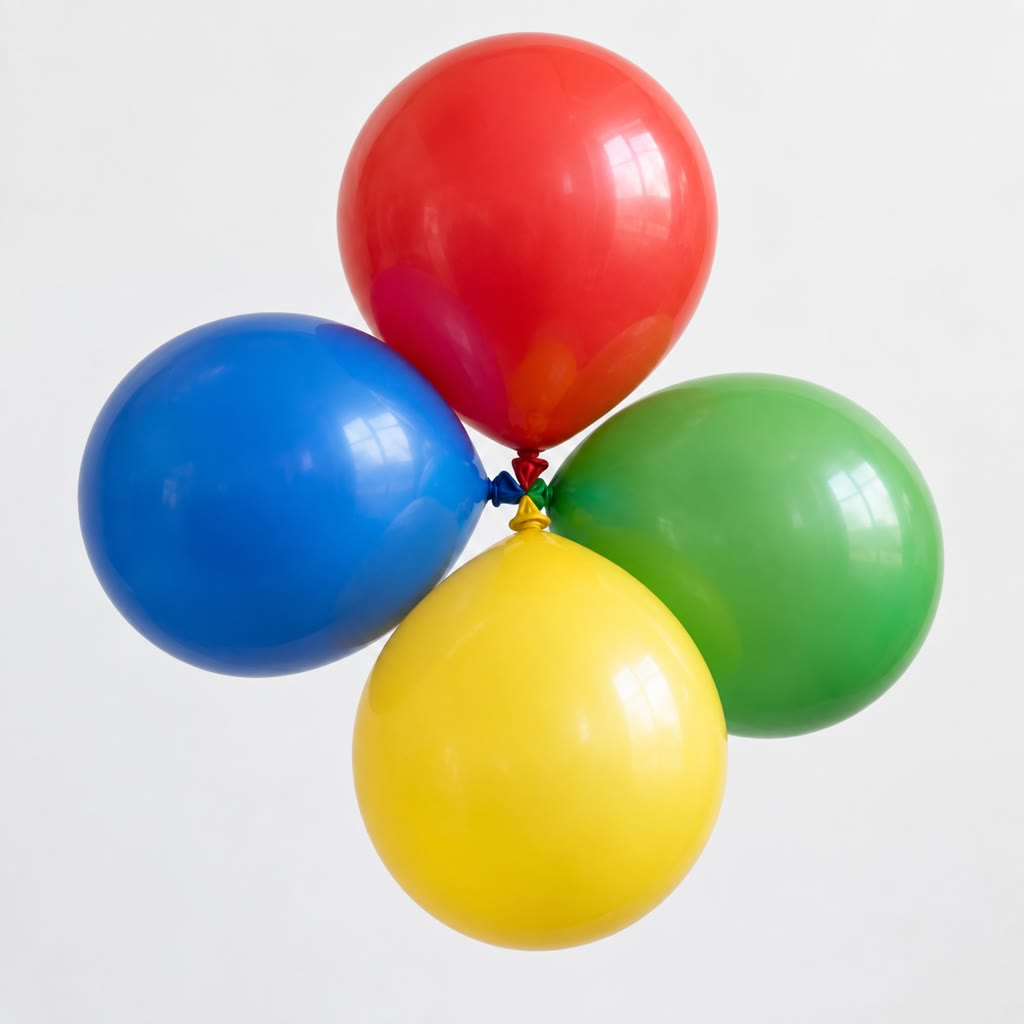
\includegraphics[width=0.38\linewidth]{images/book1/ai/g10-balloons-tetrahedron.jpg}

{\small Cuatro globos atados se empujan unos a otros para alejarse lo
más posible; en el espacio apuntan a los vértices de un tetraedro, como
los cuatro pares de \omterm{def:g9:inside-the-atom:nucleus}{electrones} alrededor de un \omterm{def:g7:atoms-and-molecules:atom}{átomo} de carbono.}
\end{omfigure}

\section{Dibujar las moléculas en el espacio}

\begin{notation}[Cuñas y trazos discontinuos]\label{not:g10:lewis-and-shape:wedge}
Para dibujar una \omterm{def:g7:atoms-and-molecules:molecule}{molécula} en el espacio sobre un papel plano, un enlace
situado en el plano del papel se dibuja con un trazo normal, un enlace
que apunta hacia el lector con una cuña llena, y un enlace que se aleja
con una cuña discontinua. El metano se dibuja entonces como aparece
debajo: dos enlaces en el plano, uno hacia el lector y otro alejándose
de él.
\begin{center}
\chemfig{C(-[2]H)(-[4]H)(<[7]H)(<:[5]H)}
\end{center}
\end{notation}

\section{Ejercicios}

\begin{exercise}[$\star$]\label{exo:g10:lewis-and-shape:1}
¿Qué es un \omterm{def:g10:lewis-and-shape:covalent-bond}{enlace covalente}? ¿Qué es un \omterm{def:g10:lewis-and-shape:lone-pair}{par no enlazante}?
\end{exercise}

\begin{exercise}[$\star$]\label{exo:g10:lewis-and-shape:2}
¿Cuántos \omterm{def:g10:lewis-and-shape:covalent-bond}{enlaces covalentes} forman habitualmente el hidrógeno, el
carbono, el nitrógeno y el oxígeno? Explícalo con las \omterm{def:g10:electron-shells:octet}{reglas del octeto}
y del dúo.
\end{exercise}

\begin{exercise}[$\star$]\label{exo:g10:lewis-and-shape:3}
Dibuja la \omterm{def:g10:lewis-and-shape:lewis-structure}{estructura de Lewis} del cloruro de hidrógeno, \ce{HCl}, y
cuenta los \omterm{def:g9:inside-the-atom:nucleus}{electrones} que rodean al cloro.
\end{exercise}

\begin{exercise}[$\star$]\label{exo:g10:lewis-and-shape:4}
¿Cuántos \omterm{def:g10:electron-shells:valence}{electrones de valencia} tiene en total la \omterm{def:g7:atoms-and-molecules:molecule}{molécula} \ce{NH3}?
¿Cuántos pares?
\end{exercise}

\begin{exercise}[$\star$]\label{exo:g10:lewis-and-shape:5}
Da la forma de \ce{CH4}, \ce{NH3}, \ce{H2O} y \ce{CO2}.
\end{exercise}

\begin{exercise}[$\star\star$]\label{exo:g10:lewis-and-shape:6}
Dibuja la \omterm{def:g10:lewis-and-shape:lewis-structure}{estructura de Lewis} del sulfuro de hidrógeno, \ce{H2S} (el
azufre está en el grupo del oxígeno), y predice su forma.
\end{exercise}

\begin{exercise}[$\star\star$]\label{exo:g10:lewis-and-shape:7}
Dibuja la \omterm{def:g10:lewis-and-shape:lewis-structure}{estructura de Lewis} del nitrógeno, \ce{N2}, siguiendo el
método paso a paso.
\end{exercise}

\begin{exercise}[$\star\star$]\label{exo:g10:lewis-and-shape:8}
Dibuja la \omterm{def:g10:lewis-and-shape:lewis-structure}{estructura de Lewis} del metanol, \ce{CH3OH}, y da la forma
alrededor del carbono y alrededor del oxígeno.
\end{exercise}

\begin{exercise}[$\star\star$]\label{exo:g10:lewis-and-shape:9}
¿Por qué el \ce{CO2} es lineal y el \ce{H2O} angular, si los dos tienen
un \omterm{def:g7:atoms-and-molecules:atom}{átomo} central unido a otros dos?
\end{exercise}

\begin{exercise}[$\star\star$]\label{exo:g10:lewis-and-shape:10}
Dibuja la \omterm{def:g10:lewis-and-shape:lewis-structure}{estructura de Lewis} del eteno, \ce{C2H4}, y da la forma
alrededor de cada \omterm{def:g7:atoms-and-molecules:atom}{átomo} de carbono.
\end{exercise}

\begin{exercise}[$\star\star$]\label{exo:g10:lewis-and-shape:11}
Dibuja la \omterm{def:g10:lewis-and-shape:lewis-structure}{estructura de Lewis} del tetraclorometano, \ce{CCl4}, y
predice su forma.
\end{exercise}

\begin{exercise}[$\star\star\star$]\label{exo:g10:lewis-and-shape:12}
Dos \omterm{def:g7:atoms-and-molecules:molecule}{moléculas} tienen la fórmula \ce{C2H6O}. Dibuja una \omterm{def:g10:lewis-and-shape:lewis-structure}{estructura de
Lewis} para cada una (una tiene un enlace O--H, y la otra, una cadena
C--O--C).
\end{exercise}

\begin{exercise}[$\star\star\star$]\label{exo:g10:lewis-and-shape:13}
Explica, con los \omterm{def:g10:lewis-and-shape:lone-pair}{pares no enlazantes}, por qué el ángulo del amoniaco
(\ang{106.7}) es menor que el del metano (\ang{109.5}), y el del agua
(\ang{104.5}), menor todavía.
\end{exercise}

\begin{exercise}[$\star\star\star$]\label{exo:g10:lewis-and-shape:14}
Dibuja la \omterm{def:g10:lewis-and-shape:lewis-structure}{estructura de Lewis} del cianuro de hidrógeno, \ce{HCN}, y la
del metanal, \ce{CH2O}, y da sus formas.
\end{exercise}

\begin{exercise}[$\star\star\star$]\label{exo:g10:lewis-and-shape:15}
El ozono, \ce{O3}, es una cadena de tres \omterm{def:g7:atoms-and-molecules:atom}{átomos} de oxígeno. Cuenta sus
pares de valencia y dibuja una \omterm{def:g10:lewis-and-shape:lewis-structure}{estructura de Lewis} en la que todos los
oxígenos tengan su octeto (un \omterm{def:g10:lewis-and-shape:multiple-bond}{enlace doble} y uno sencillo). Predice si la
\omterm{def:g7:atoms-and-molecules:molecule}{molécula} es lineal o angular.
\end{exercise}

\section{Problema: Una molécula en un cubo}

\begin{problem}[{Problema de fin de semana --- diseñar las bolas de
carbono de un juego de modelos moleculares: ¿con qué ángulo hay que
taladrar los agujeros?}]
\label{pb:g10:lewis-and-shape:1}
% ledger: ang:H2O, ang:NH3
Una empresa fabrica juegos de modelos moleculares. Las bolas negras de
carbono deben tener cuatro agujeros, para que el metano, el etano y las
demás \omterm{def:g7:atoms-and-molecules:molecule}{moléculas} del carbono salgan con la forma correcta. El ingeniero
usa un truco: un tetraedro regular cabe dentro de un cubo, con sus
cuatro vértices en cuatro vértices del cubo, sin que haya dos en la misma
arista.

\medskip
\noindent\textbf{Parte I --- \omterm{def:g10:lewis-and-shape:lewis-structure}{Estructuras de Lewis}.}
\begin{enumerate}
  \item Dibuja las \omterm{def:g10:lewis-and-shape:lewis-structure}{estructuras de Lewis} del metano \ce{CH4}, el amoniaco
        \ce{NH3} y el agua \ce{H2O}.
  \item ¿Cuántos grupos de \omterm{def:g9:inside-the-atom:nucleus}{electrones} rodean el \omterm{def:g7:atoms-and-molecules:atom}{átomo} central en cada
        una?
  \item ¿Cuántos de ellos son \omterm{def:g10:lewis-and-shape:lone-pair}{pares no enlazantes}?
  \item ¿Por qué una bola de carbono necesita cuatro agujeros, y una bola
        de oxígeno (para el agua), solo dos?
  \item Un modelo de etano, \ce{C2H6}, usa dos bolas de carbono. Dibuja
        su \omterm{def:g10:lewis-and-shape:lewis-structure}{estructura de Lewis}. ¿Cuántas varillas unen las dos bolas de
        carbono, y cuántas bolas de hidrógeno hacen falta?
\end{enumerate}

\medskip
\noindent\textbf{Parte II --- Formas.}
\begin{enumerate}[resume]
  \item Da la forma de cada una de las tres \omterm{def:g7:atoms-and-molecules:molecule}{moléculas}.
  \item Los ángulos medidos son de \ang{106.7} en el amoniaco y de
        \ang{104.5} en el agua. Explica por qué son menores que el
        ángulo del metano.
  \item ¿Por qué la bola de oxígeno para el agua no puede ser
        simplemente una bola de carbono con dos agujeros vacíos, si el
        juego tiene que mostrar el ángulo real?
  \item En el dióxido de carbono, el \omterm{def:g7:atoms-and-molecules:atom}{átomo} de carbono forma dos \omterm{def:g10:lewis-and-shape:multiple-bond}{enlaces
        dobles}. ¿Qué ángulo debe separarlos en un modelo?
\end{enumerate}

\medskip
\noindent\textbf{Parte III --- El cubo.}
Toma un cubo de arista $a$. El \omterm{def:g7:atoms-and-molecules:atom}{átomo} de carbono está en su centro; los
cuatro \omterm{def:g7:atoms-and-molecules:atom}{átomos} de hidrógeno ocupan cuatro vértices del cubo, sin que haya
dos en la misma arista.
\begin{enumerate}[resume]
  \item Muestra que dos cualesquiera de estos \omterm{def:g7:atoms-and-molecules:atom}{átomos} de hidrógeno están
        en los dos extremos de una diagonal de una cara del cubo. Con el
        teorema de Pitágoras, calcula la distancia entre ellos en función
        de $a$.
  \item La diagonal del cubo entero (de un vértice al vértice opuesto)
        mide $a\sqrt{3}$. Deduce la distancia del \omterm{def:g7:atoms-and-molecules:atom}{átomo} de carbono a un
        \omterm{def:g7:atoms-and-molecules:atom}{átomo} de hidrógeno.
  \item Toma $a = \qty{1}{cm}$ en un modelo: da las dos distancias en
        centímetros, con dos decimales.
  \item ¿Por qué son iguales las cuatro distancias C--H?
\end{enumerate}

\medskip
\noindent\textbf{Parte IV --- El ángulo.}
El \omterm{def:g7:atoms-and-molecules:atom}{átomo} de carbono C y dos \omterm{def:g7:atoms-and-molecules:atom}{átomos} de hidrógeno H$_1$ y H$_2$ forman un
triángulo isósceles. Sea M el punto medio de H$_1$H$_2$.
\begin{enumerate}[resume]
  \item Explica por qué el triángulo C\,M\,H$_1$ es rectángulo en M.
  \item Calcula, en este triángulo rectángulo, el seno del ángulo
        $\widehat{\text{M\,C\,H}_1}$, la mitad del ángulo H--C--H.
  \item Deduce el semiángulo y, después, el ángulo H--C--H, con un
        decimal.
  \item Compáralo con el ángulo de la tabla de este capítulo.
  \item Indica el ángulo con el que hay que taladrar los agujeros de una
        bola de carbono.
\end{enumerate}
\end{problem}
